\documentclass[12pt]{article}
\usepackage{graphicx}
\usepackage[margin=1in]{geometry}
\usepackage{setspace}
\usepackage{booktabs}
\usepackage{hyperref}
\usepackage[
backend=biber,
style=alphabetic,
]{biblatex}
\addbibresource{references.bib}
\usepackage{amsmath} 


\title{Predicting the Housing Market using \\ Linear Regression}

\author{Garrick Ho\\
  Jun Yan\\[1ex]
  Department of Statistics\\
  University of Connecticut\\
}

\begin{document}

\maketitle
\doublespace

\begin{abstract}
With the housing market fluctuating every year, many real estate owners and businesses face a problem with gaining an accurate representation of the future of the housing market. Lots of people do not know much about the market, so they will go to real estate owners or businesses to learn more about the market. And then see what the market is at and if it is the right time to buy a house. If real estate owners and businesses are able to gain more accuracy in predicting the housing market, they will be able to help more people and possibly gain more business. Not only can this benefit the consumers, the builders are able to move with the market and have a better understanding of it. This paper aims to construct a robust linear regression model by using machine learning techniques to predict housing costs accurately. By leveraging natural language processing, the linear regression model analyzes home property descriptions and extracts vital insights that significantly contribute to precise pricing predictions. This paper ends with an explanation of the limitations of this study and potential future works that can be done.

\bigskip
\noindent{\sc Keywords}:
housing market;
natural language processing;
linear regression;
model predictions


\end{abstract}

\section{Introduction}
\label{sec:intro}

% Why does it matter?
% What has already been done?
% What is new?



% An overview of the topic
% Existing works
% Why are existing methods not sufficient? What are the elements of an attractive solution?
% Contributions

% A roadmap
The rest of the paper is organized in the following way.
Beginning with the overall introduction located in Section~\ref{sec:intro}.
A brief introduction about the data will be shown in Section~\ref{sec:data}. Here, the variables will be described and explained how they contribute to the research question.
Then, the methodology used in this paper will be explained in Section~\ref{sec:meth}.
Next, the simulation will be reported in Section~\ref{sec:sim}. This section will present the results from the model and have further analysis with tables and figures.
The applications of the results found will be in Section~\ref{sec:app}. More in-depth analysis of how the results can be applied to the real world will be in this section.
Finally, the discussion part for this paper will be in Section~\ref{sec:disc}. The limitations of the current study and future direction will be discussed here.
All the references used in this paper will be included in Section~\ref{sec:refer}.


\section{Data}
\label{sec:data}

% Who collected the data (source)?
% How was the data collected? Sampling frame? Sampling approach?
% What period or range does the data cover?
% Why does the data help answer the research question?
% What exploratory analyses are done (descriptives, visualization, etc.)?

The data that will be used for this study was sourced from \href{https://www.kaggle.com/code/ashydv/housing-price-prediction-linear-regression/input}{Kaggle}. It is a data set that contains \(n = 545\) observations (different house samples) of thirteen variables, seven of which are categorical variables and six are numerical variables. The data set contains features and corresponding labels for training and testing a Multiple Linear Regression (MLR) model to predict the house cost.
The data was explored and visualized using the pandas library in Python. For the columns that were strings, they have been transformed into an integer data type so that they can be read in the model. More specifically, the 'furnishingstatus' column was broken down into three different columns. One for furnished, one for semi-furnished, and lastly one for unfurnished. 

\begin{table}
\caption{Data Description}
  \label{tab:rv}
\begin{tabular}{llll}
  \toprule
Variable & Data Type & Instance & Purpose \\
  \midrule
price & Int & 13300000 & \(Y\) \\ 
area & Int & 7420 & \(X_{n}\) \\ 
bedrooms & Int & 4 & \(X_{n}\) \\ 
bathrooms & Int & 2 & \(X_{n}\) \\ 
stories & Int & 3 & \(X_{n}\) \\ 
mainroad & Str & yes, no & \(X_{n}\) \\
guestroom & Str & yes, no & \(X_{n}\) \\
basement & Str & yes, no & \(X_{n}\) \\
hotwaterheating & Str & yes, no & \(X_{n}\) \\
airconditioning & Str & yes, no & \(X_{n}\) \\
parking & Int & 2 & \(X_{n}\) \\
prefarea & Str & yes, no & \(X_{n}\) \\
furnishingstatus & Str & furnished, semi-furnished, unfurnished & \(X_{n}\) \\
   \bottomrule
\end{tabular}\par
\bigskip
In Table~\ref{tab:rv}, the 'variable' column shows the names of all the variables that are in the dataset. The 'Data Type' column shows the data type of each variable in the dataset. Note that 'Int' means integer and 'Str' means string. The 'Instance' column shows an example of what a data point for that column would look like. The 'Purpose' column shows the importance of each variable to the machine learning step.
\end{table}

\begin{figure}
    \caption{Categorical Variable Plots}
    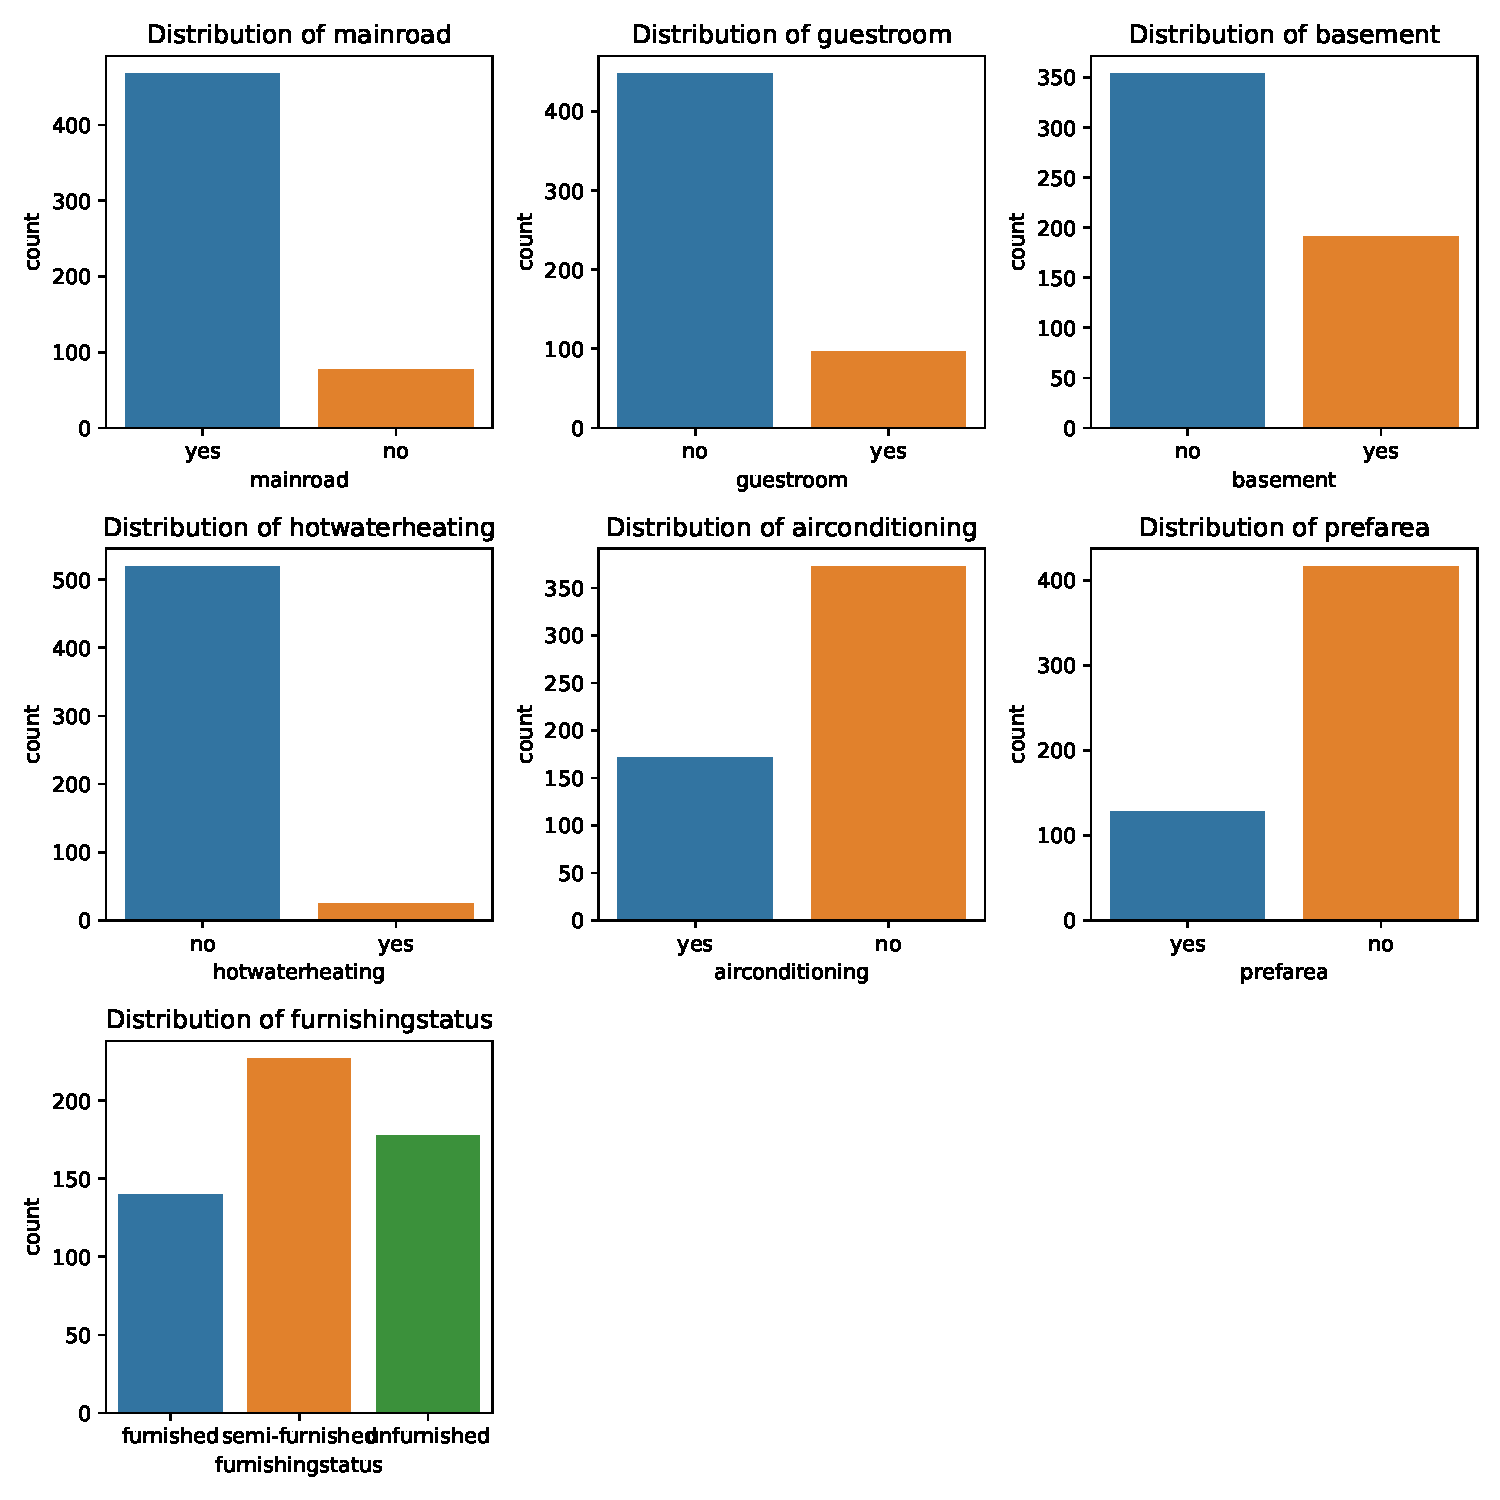
\includegraphics[width=1\textwidth]{categorical_plots.pdf}
    \label{fig:categorical_plots}
In figure~\ref{fig:categorical_plots}, the plots show the distributions for all the categorical variables. Most of the houses in this data set are located near a main road. Only one-fifth of the houses have a room for guests. For the basement category, two-fifths of them have one. Almost none of the houses have hot water heating. There is air conditioning in about two-fifths of the data. About one-fifth of the houses are located in a preferred area. And lastly, the house can come either furnished, semi-furnished, or unfurnished. Most of the house came semi-furnished, next being unfurnished and then fully furnished. 
\end{figure}

\begin{figure}
    \caption{Numerical Variable Plots}
    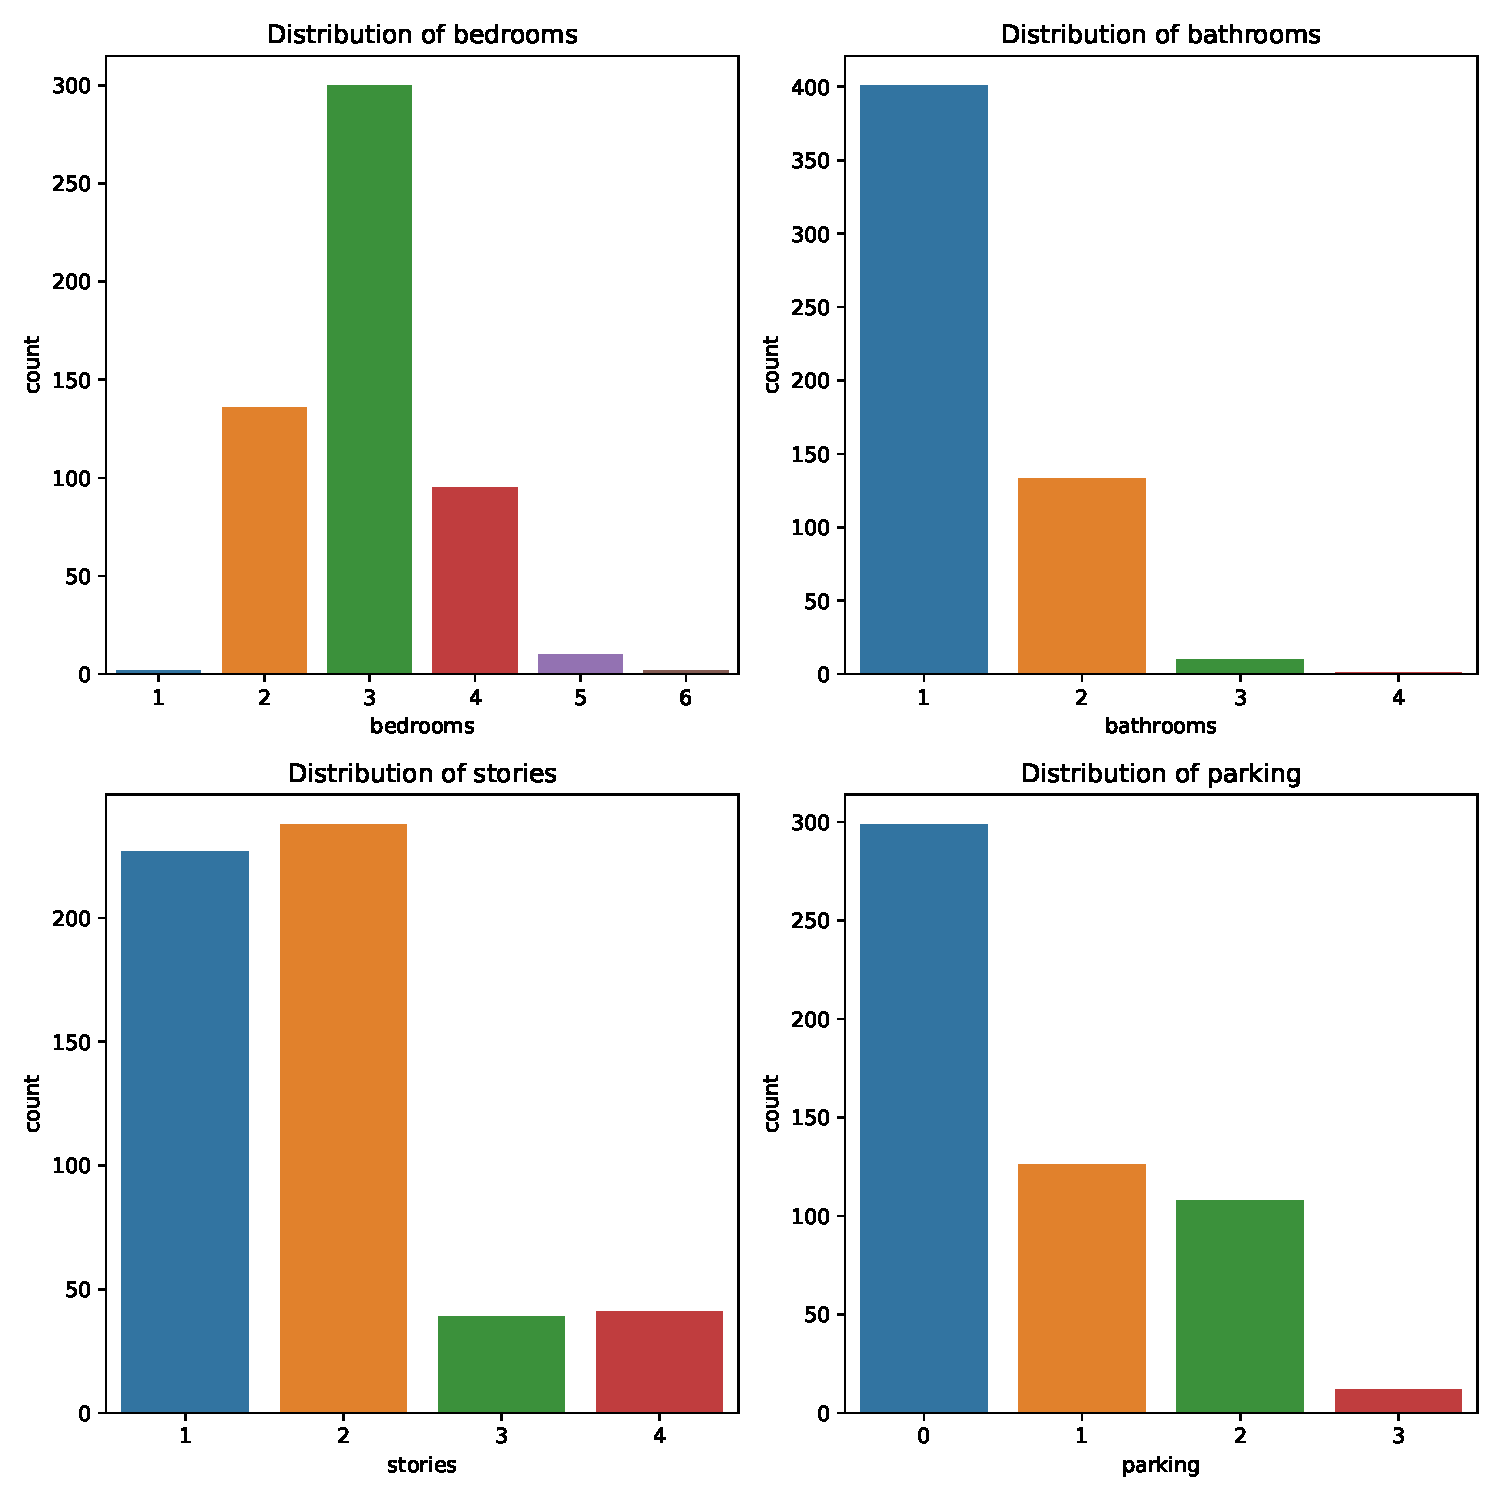
\includegraphics[width=1\textwidth]{numerical_plots.pdf}
    \label{fig:numberical_plots}
In figure~\ref{fig:numberical_plots}, four different plots are shown to display the distribution of the numerical variables in the data. The average number of bedrooms in these homes is three, with two being the second most. For the number of bathrooms, the majority of homes have one. About half of the homes in the data are one-story homes while about the other half are two stories. For parking, most of them have no parking spots. A few of them have one or two parking spots. 
\end{figure}


\bigskip
\bigskip


\section{Methods}
\label{sec:meth}

% Establish notation.
% What are the observed data?
% What are the models?
% What are the parameters to be estimated?
% How are the point estimators obtained?
% How are the uncertainty (standard errors) of the point estimators assessed?
% How are the variances of the point estimators estimated?
% How are the null distribution of the testing statistics established?
% Clearly state the assumptions and claims of theoretical results.

\begin{equation}
  \label{eq:Multi}
  Y = \beta_{0} + \beta_{1}X_{1} + \beta_{2}X_{2} + ... + \beta_{n}X_{n} + \epsilon
\end{equation}

Equation~\ref{eq:Multi} is the Multiple Linear Regression model being used. \(Y\) is the dependent variable, also known as the value that is being predicted. In this case, it would be the cost of a house. \(X_{n}\) is the independent variable, which is the characteristics of the house that are used to predict the house cost. \(\beta_{n}\) is the average amount by which the dependent variable increases and decreases depending on when the independent variable increases one standard deviation. When all the other independent variables are held constant. \(\beta_{0}\) represents the value of the dependent variable when all the independent variables are equal to zero. \(\epsilon\) is the error term which represents the margin of error within the linear regression model. \cite{uyanik2013}


\section{Simulation}
\label{sec:sim}

% Aims
% Data generating mechanism
% Estimand/target of analysis
% Methods
% Performance measures

\begin{align}\label{eq:R2}
\begin{split}
    R^2 &= 1 - \frac{\text{sum squared regression (SSR)}}{\text{total sum of squares (SST)}}, \\
    &= 1-\frac{\sum(y_i - \hat{y_i})^2 }{\sum(y_i - \Bar{y})^2} 
\end{split}
\end{align}

Equation~\ref{eq:R2} is the formula for R-squared. R-squared is a measure of the goodness of fit of a model. The sum squared regression is the sum of the residuals squared and the total sum of squares is the sum of the distance the data is away from the mean all squared. It is a percentage that takes the values between 0 and 1. If the percentage is 1, then the variation in the \(y\) values is accounted for by the \(x\) values. If the percentage is 0, then none of the variations of the \(y\) values is accounted for by the \(x\) values. \cite{kasuya2018}

\section{Application}
\label{sec:app}

% Report the statistical analyses in tables/figures.
% When summarizing from tables/figures, paint the big picture, rather than reiterating all of the little details.
% Discussions to link the analyses 

\section{Discussion and Conclusion}
\label{sec:disc}

% A summary, again, of the contributions of the research.
% The research question posed as the `need’ of the introduction must be answered here (Zeiger 2000).
% Limitations of the current study
% Future directions.


\section{References}
\label{sec:refer}

% Every reference cited in the paper should appear here.
% References not cited should not appear here.
% All are automatically taken care of by BibTeX.
% Styles are controlled by bib style (.bst file).


\cite{singh2021}
\cite{alfiyantin2017}
\cite{uyanik2013}

\medskip

\printbibliography[title={References}]


\end{document}
